% Options for packages loaded elsewhere
\PassOptionsToPackage{unicode}{hyperref}
\PassOptionsToPackage{hyphens}{url}
\PassOptionsToPackage{dvipsnames,svgnames,x11names}{xcolor}
%
\documentclass[
  ignorenonframetext,
]{beamer}
\usepackage{pgfpages}
\setbeamertemplate{caption}[numbered]
\setbeamertemplate{caption label separator}{: }
\setbeamercolor{caption name}{fg=normal text.fg}
\beamertemplatenavigationsymbolsempty
% Prevent slide breaks in the middle of a paragraph
\widowpenalties 1 10000
\raggedbottom
\setbeamertemplate{part page}{
  \centering
  \begin{beamercolorbox}[sep=16pt,center]{part title}
    \usebeamerfont{part title}\insertpart\par
  \end{beamercolorbox}
}
\setbeamertemplate{section page}{
  \centering
  \begin{beamercolorbox}[sep=12pt,center]{part title}
    \usebeamerfont{section title}\insertsection\par
  \end{beamercolorbox}
}
\setbeamertemplate{subsection page}{
  \centering
  \begin{beamercolorbox}[sep=8pt,center]{part title}
    \usebeamerfont{subsection title}\insertsubsection\par
  \end{beamercolorbox}
}
\AtBeginPart{
  \frame{\partpage}
}
\AtBeginSection{
  \ifbibliography
  \else
    \frame{\sectionpage}
  \fi
}
\AtBeginSubsection{
  \frame{\subsectionpage}
}
\usepackage{amsmath,amssymb}
\usepackage{lmodern}
\usepackage{iftex}
\ifPDFTeX
  \usepackage[T1]{fontenc}
  \usepackage[utf8]{inputenc}
  \usepackage{textcomp} % provide euro and other symbols
\else % if luatex or xetex
  \usepackage{unicode-math}
  \defaultfontfeatures{Scale=MatchLowercase}
  \defaultfontfeatures[\rmfamily]{Ligatures=TeX,Scale=1}
\fi
% Use upquote if available, for straight quotes in verbatim environments
\IfFileExists{upquote.sty}{\usepackage{upquote}}{}
\IfFileExists{microtype.sty}{% use microtype if available
  \usepackage[]{microtype}
  \UseMicrotypeSet[protrusion]{basicmath} % disable protrusion for tt fonts
}{}
\makeatletter
\@ifundefined{KOMAClassName}{% if non-KOMA class
  \IfFileExists{parskip.sty}{%
    \usepackage{parskip}
  }{% else
    \setlength{\parindent}{0pt}
    \setlength{\parskip}{6pt plus 2pt minus 1pt}}
}{% if KOMA class
  \KOMAoptions{parskip=half}}
\makeatother
\usepackage{xcolor}
\newif\ifbibliography
\usepackage{graphicx}
\makeatletter
\def\maxwidth{\ifdim\Gin@nat@width>\linewidth\linewidth\else\Gin@nat@width\fi}
\def\maxheight{\ifdim\Gin@nat@height>\textheight\textheight\else\Gin@nat@height\fi}
\makeatother
% Scale images if necessary, so that they will not overflow the page
% margins by default, and it is still possible to overwrite the defaults
% using explicit options in \includegraphics[width, height, ...]{}
\setkeys{Gin}{width=\maxwidth,height=\maxheight,keepaspectratio}
% Set default figure placement to htbp
\makeatletter
\def\fps@figure{htbp}
\makeatother
\setlength{\emergencystretch}{3em} % prevent overfull lines
\providecommand{\tightlist}{%
  \setlength{\itemsep}{0pt}\setlength{\parskip}{0pt}}
\setcounter{secnumdepth}{-\maxdimen} % remove section numbering
\usepackage{soul}
\usepackage[T1]{fontenc}
\usepackage{amsmath}
\usepackage{listings}
\usepackage{graphicx}
\usepackage{tikz}
\usepackage{pgfplots}
\usepackage{tkz-fct}
\usepackage{comment}
\usepackage{filecontents}
\setbeamertemplate{navigation symbols}{}
\usecolortheme{crane}
\RequirePackage{etex}
\ifLuaTeX
  \usepackage{selnolig}  % disable illegal ligatures
\fi
\IfFileExists{bookmark.sty}{\usepackage{bookmark}}{\usepackage{hyperref}}
\IfFileExists{xurl.sty}{\usepackage{xurl}}{} % add URL line breaks if available
\urlstyle{same} % disable monospaced font for URLs
\hypersetup{
  pdftitle={Day 6: Calculus II, Integrals},
  pdfauthor={Sarah Moore and Jason Seawright},
  colorlinks=true,
  linkcolor={Maroon},
  filecolor={Maroon},
  citecolor={Blue},
  urlcolor={red},
  pdfcreator={LaTeX via pandoc}}

\title{Day 6: Calculus II, Integrals}
\author{Sarah Moore and Jason Seawright}
\date{Math Camp 2022}

\begin{document}
\frame{\titlepage}

\begin{frame}{Day 6 Agenda}
\protect\hypertarget{day-6-agenda}{}
\begin{itemize}
\item
  Integrals: Concept, notation, and how-to
\item
  Fundamental Theorem of Calculus
\item
  Computing Integrals: Substitution and by Parts
\item
  Advanced Rules of Integrals
\end{itemize}
\end{frame}

\begin{frame}{Let's Take a Step Back\ldots{}}
\protect\hypertarget{lets-take-a-step-back}{}
\begin{itemize}
\item
  As a reminder, a derivative provides information about the
  \emph{instantaneous rate of change} of a function.
\item
  This means we can take a given value of \(x\) and find the rate of
  change of the function at that point, so long as the function is
  continuous at \(x\). This also means we have an equation of the
  \emph{marginal rate of change}.
\item
  However, we are not always interested in just the \emph{instantaneous
  rate of change}. Instead, we may be interested in the effect of a
  function's change over the \emph{range of the function, or over a
  given interval.}
\end{itemize}
\end{frame}

\begin{frame}{Motivating Example}
\protect\hypertarget{motivating-example}{}
\begin{itemize}
\item
  Let's say a new book store opens and based on the first 100 days of
  sales we can model daily book sales given the function
  \(f(x)= 20 +ln(x)\), where \(x\) is the number of days since the
  bookstore opened.
\item
  As we know, solving for \(x\) will give us the amount of books sold on
  that particular day.
\end{itemize}

\centering

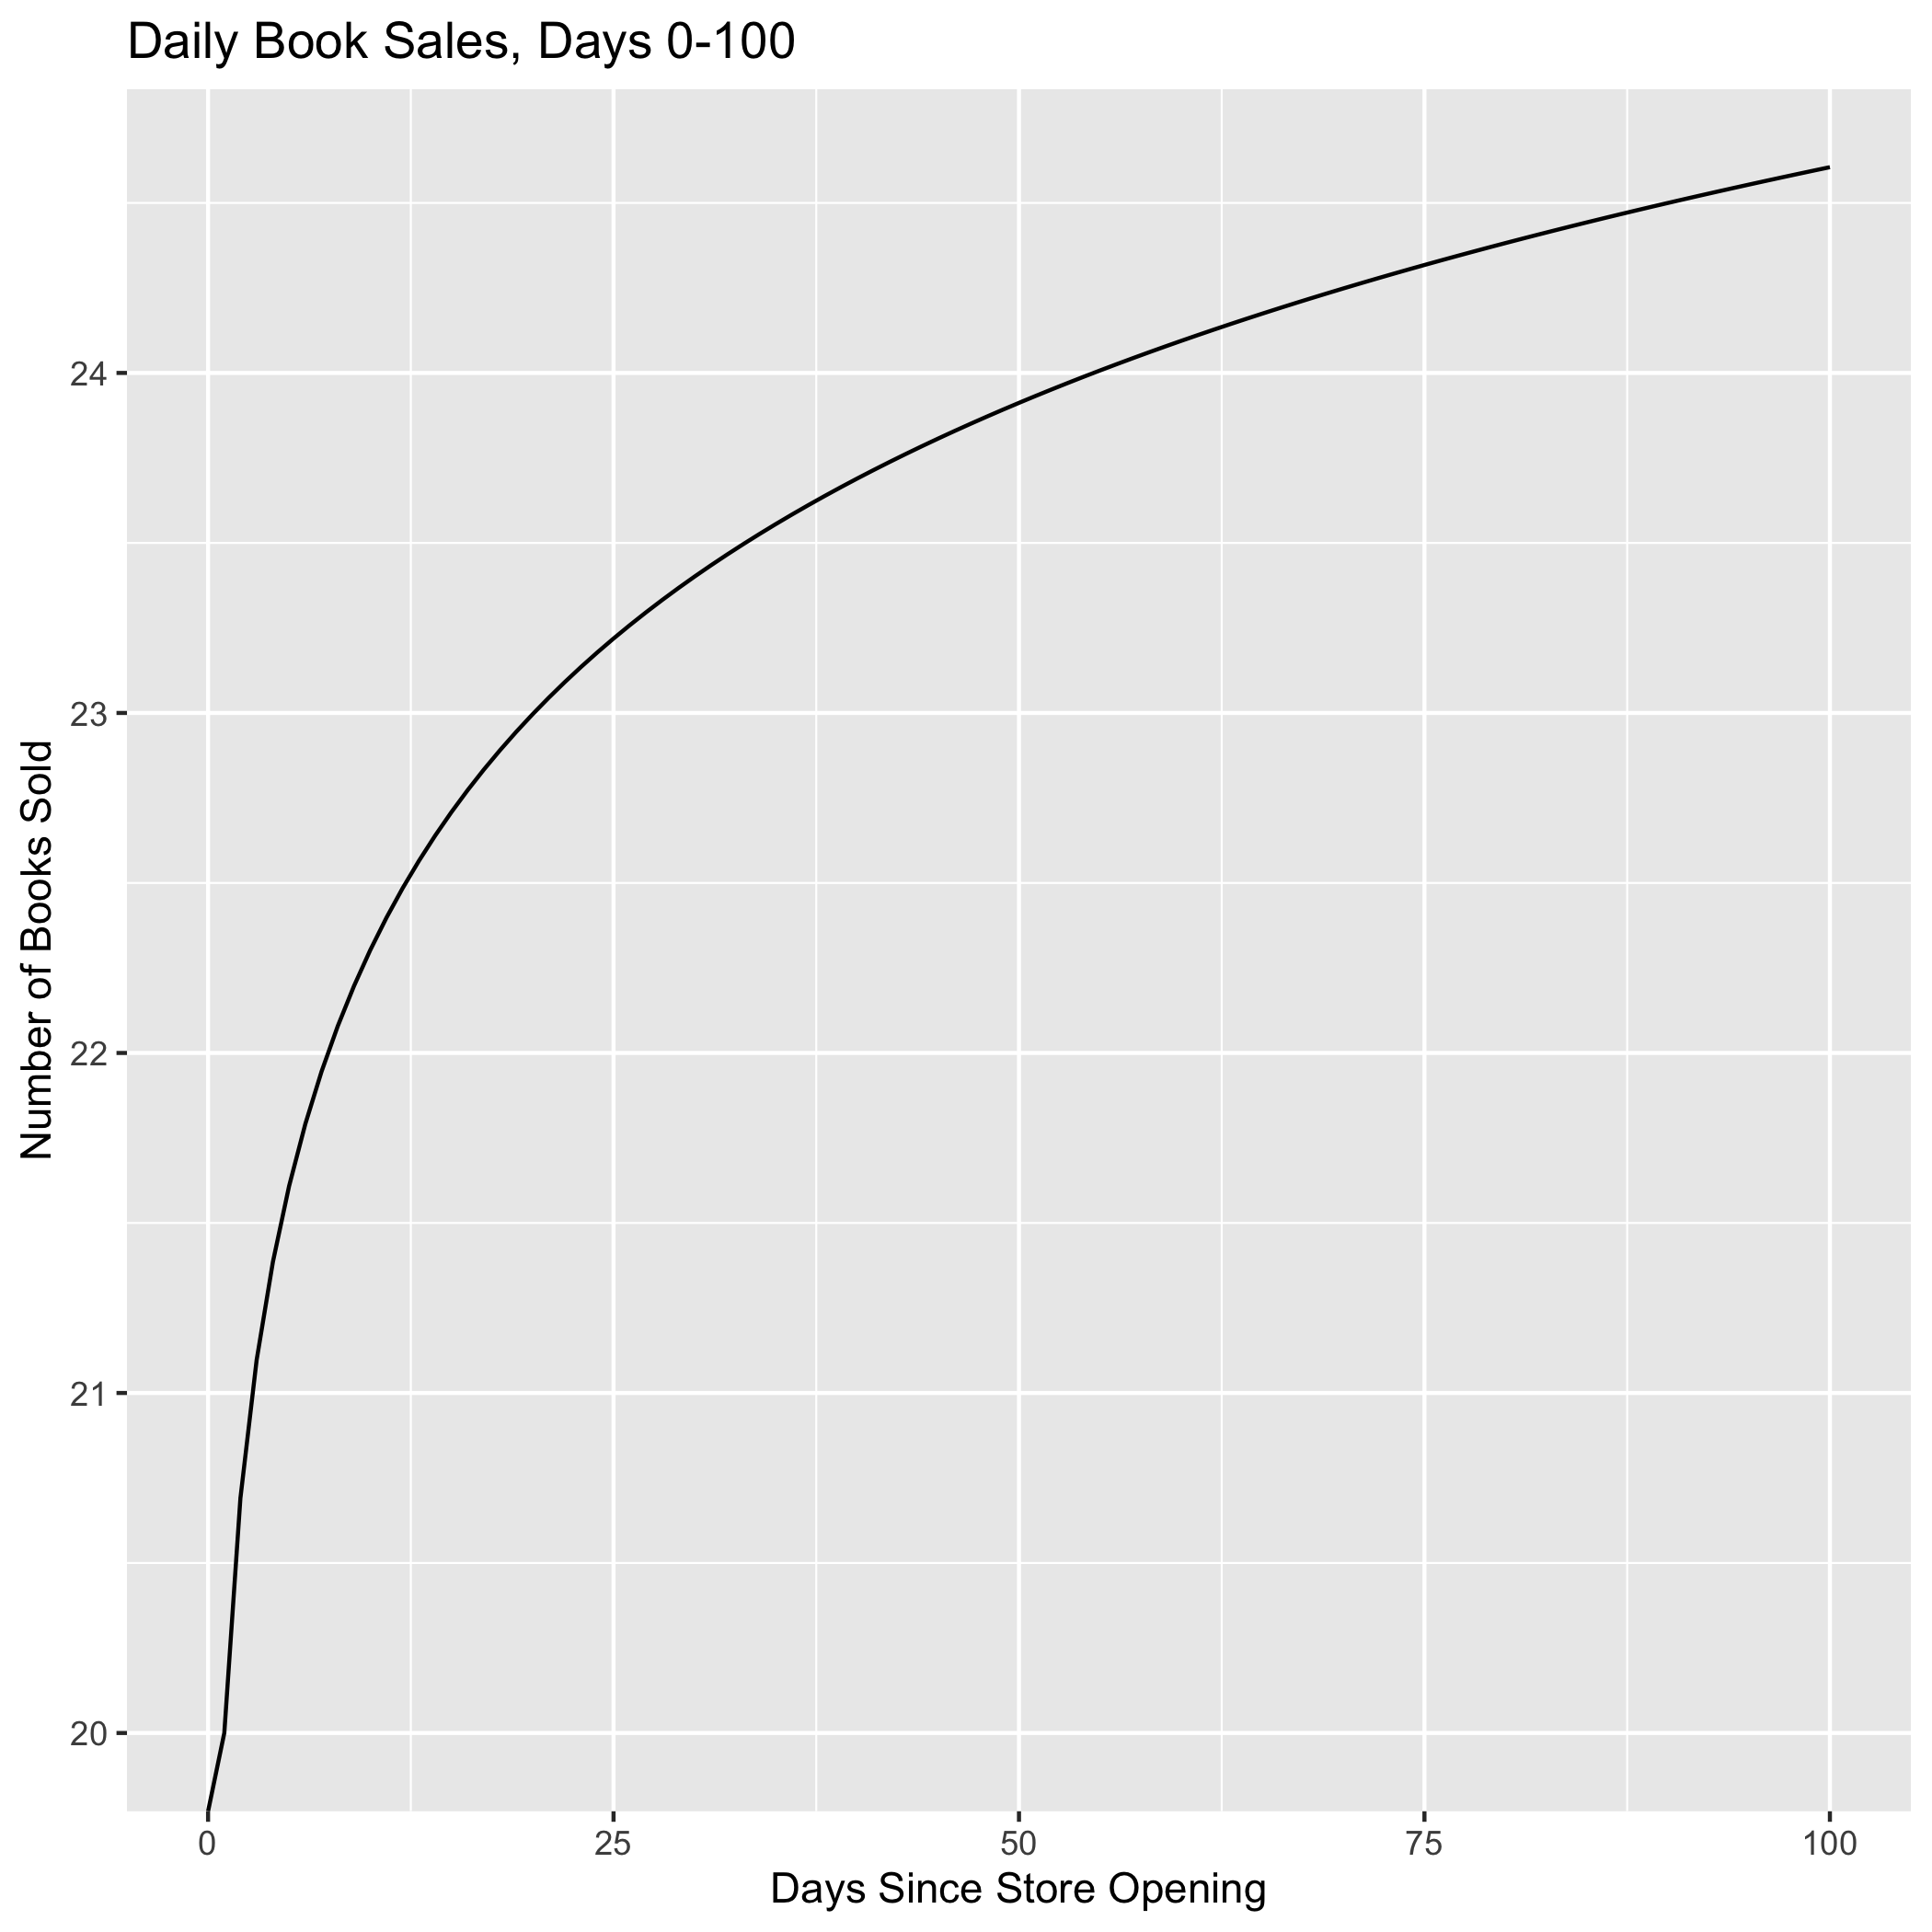
\includegraphics[width=0.4\textwidth,height=\textheight]{"~/OneDrive - Northwestern University/Teaching/2022_MathCamp/Proposed AM Slides/images/book_sales.png"}
\end{frame}

\begin{frame}{Cumulative Book Sales?}
\protect\hypertarget{cumulative-book-sales}{}
\begin{itemize}
\item
  Perhaps the bookstore is going through an audit, and instead wants to
  check for the \emph{cumulative} number of books sold for the entire
  first 100 days.
\item
  Or even more specifically, we want to know how many books were sold
  from Day 25 to Day 65.
\end{itemize}

\centering

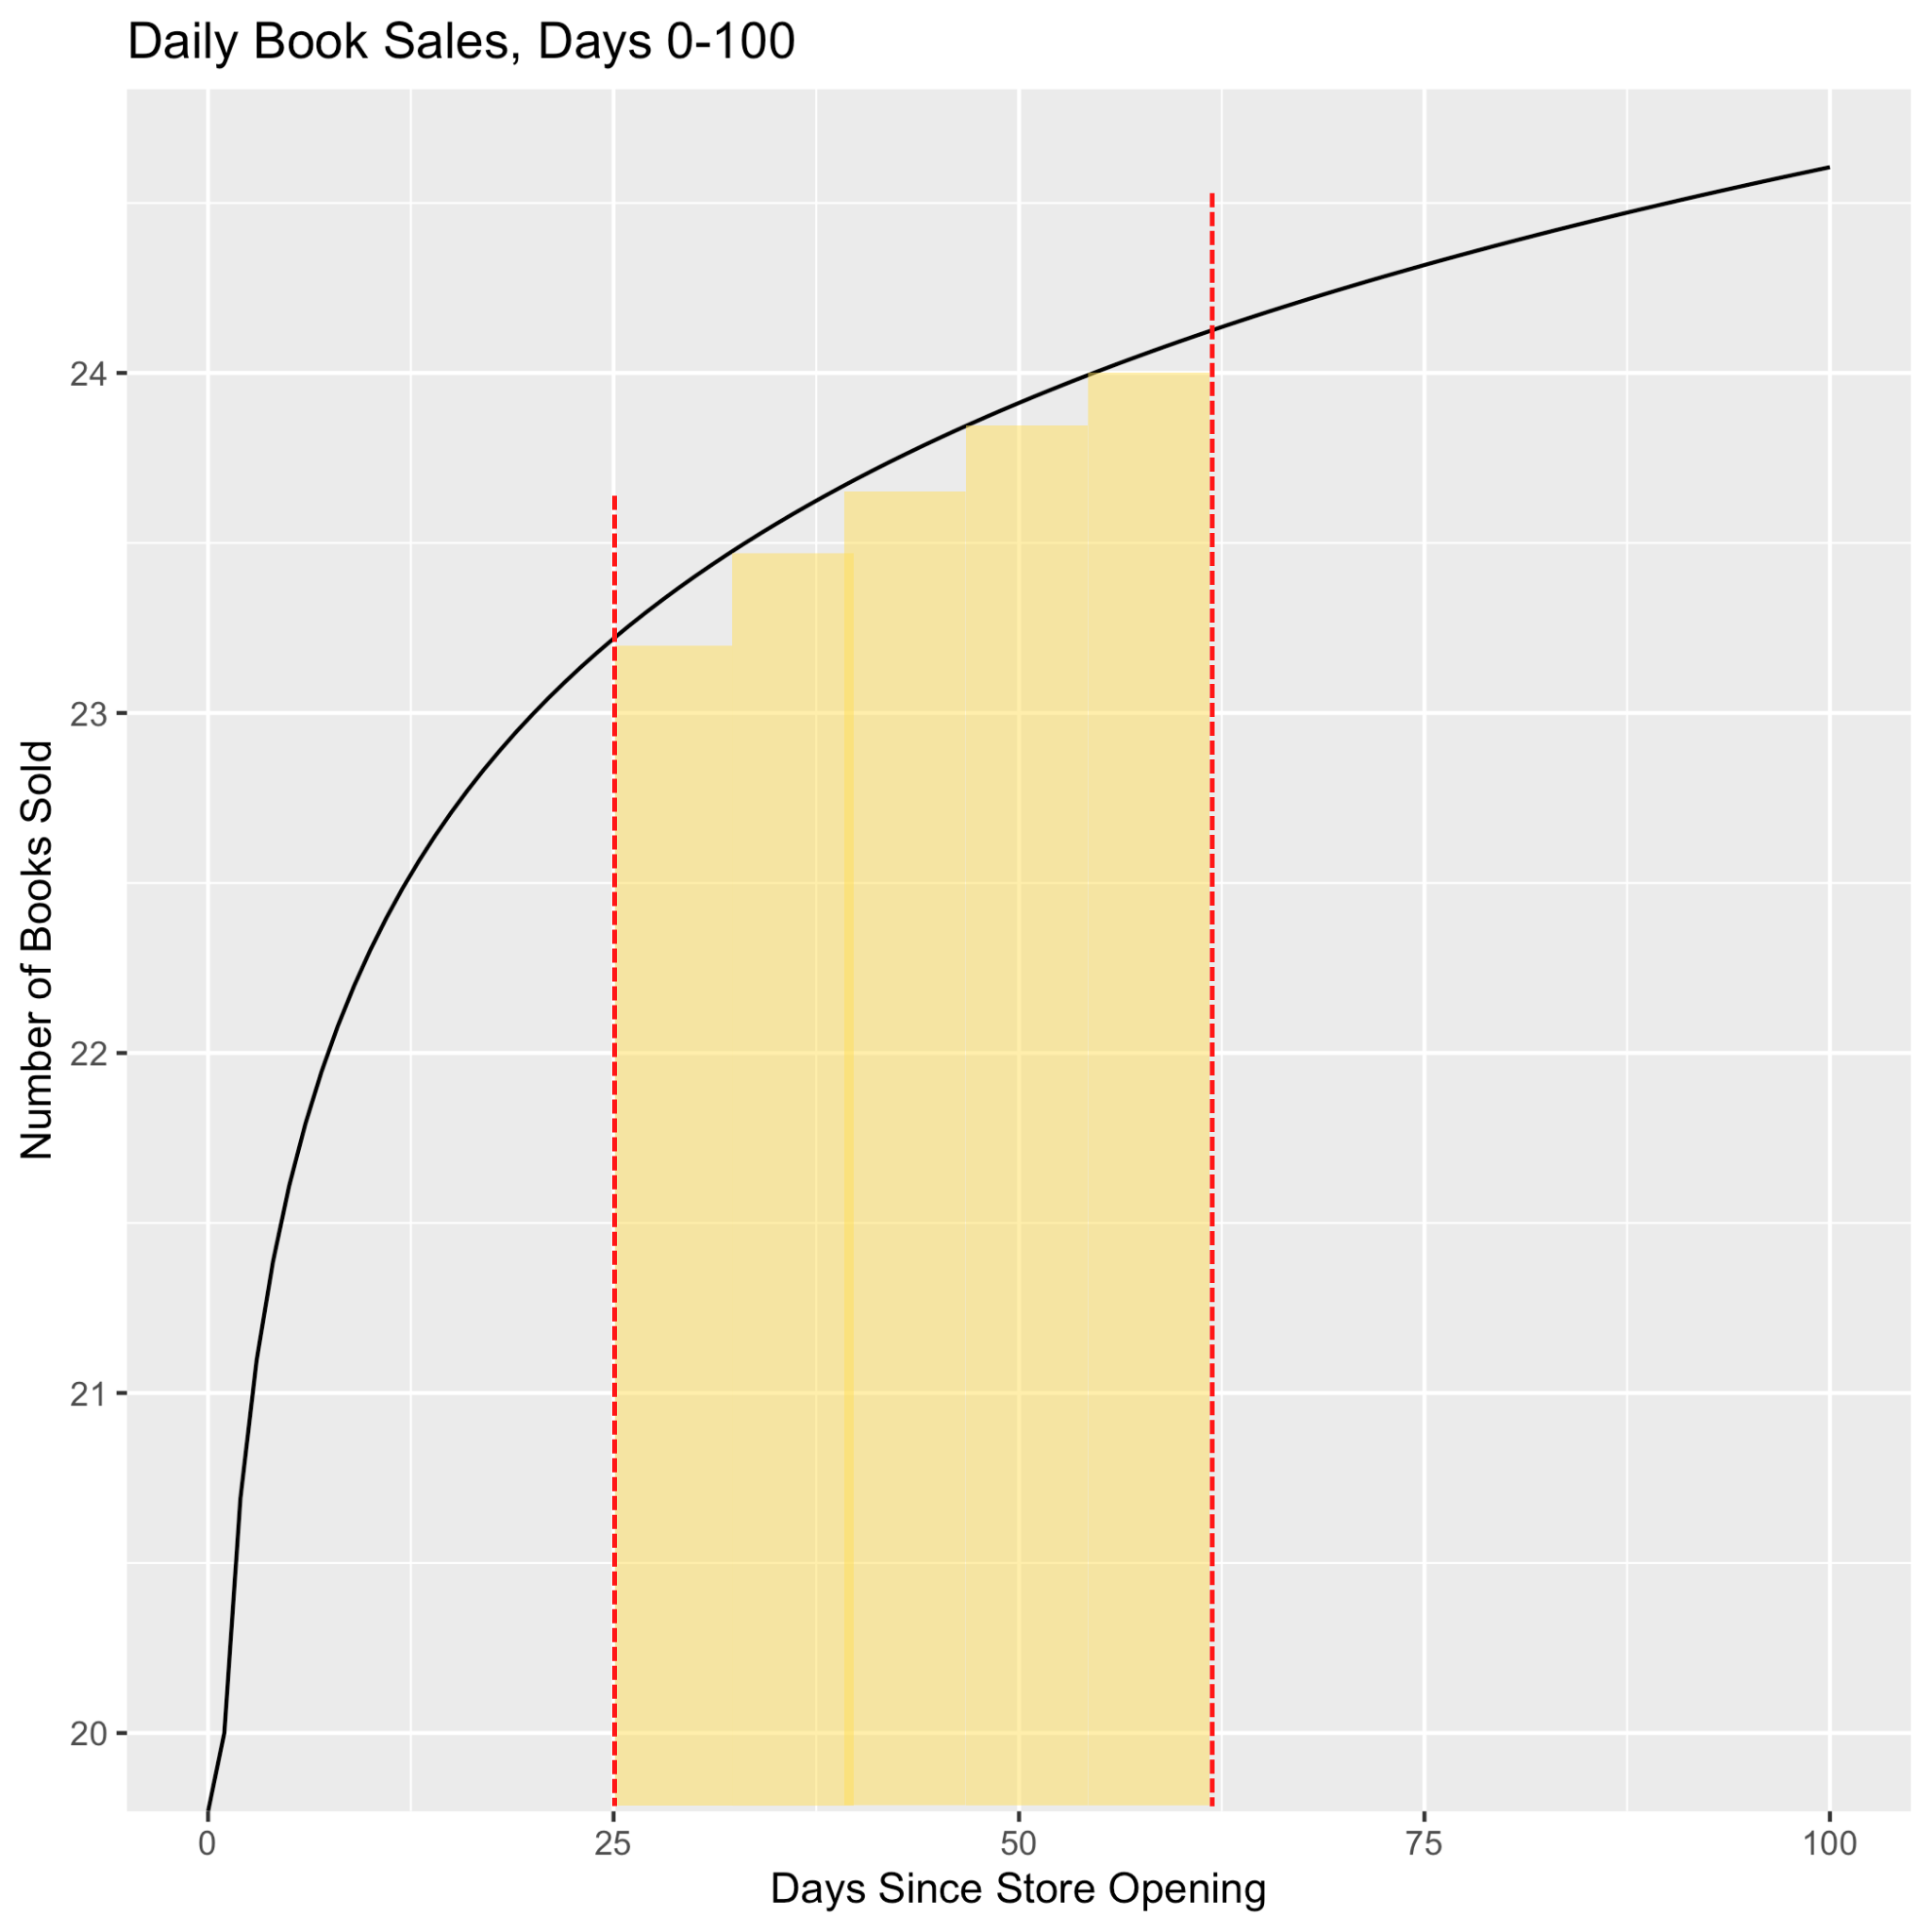
\includegraphics[width=0.5\textwidth,height=\textheight]{"~/OneDrive - Northwestern University/Teaching/2022_MathCamp/Proposed AM Slides/images/book_sales_interval.png"}
\end{frame}

\begin{frame}{Book Sales on the Interval?}
\protect\hypertarget{book-sales-on-the-interval}{}
\footnotesize

\begin{itemize}
\item
  Remember our series and summation operations? This is essentially what
  we would be required to do to find this value!
\item
  We \emph{could} solve for \(x\) for each point in the interval and
  then add these all up. To make our estimate more accurate, we would
  have to break up the intervals between each \(x\) and sum those
  together-- making the interval smaller and smaller to achieve higher
  precision.
\end{itemize}

\centering

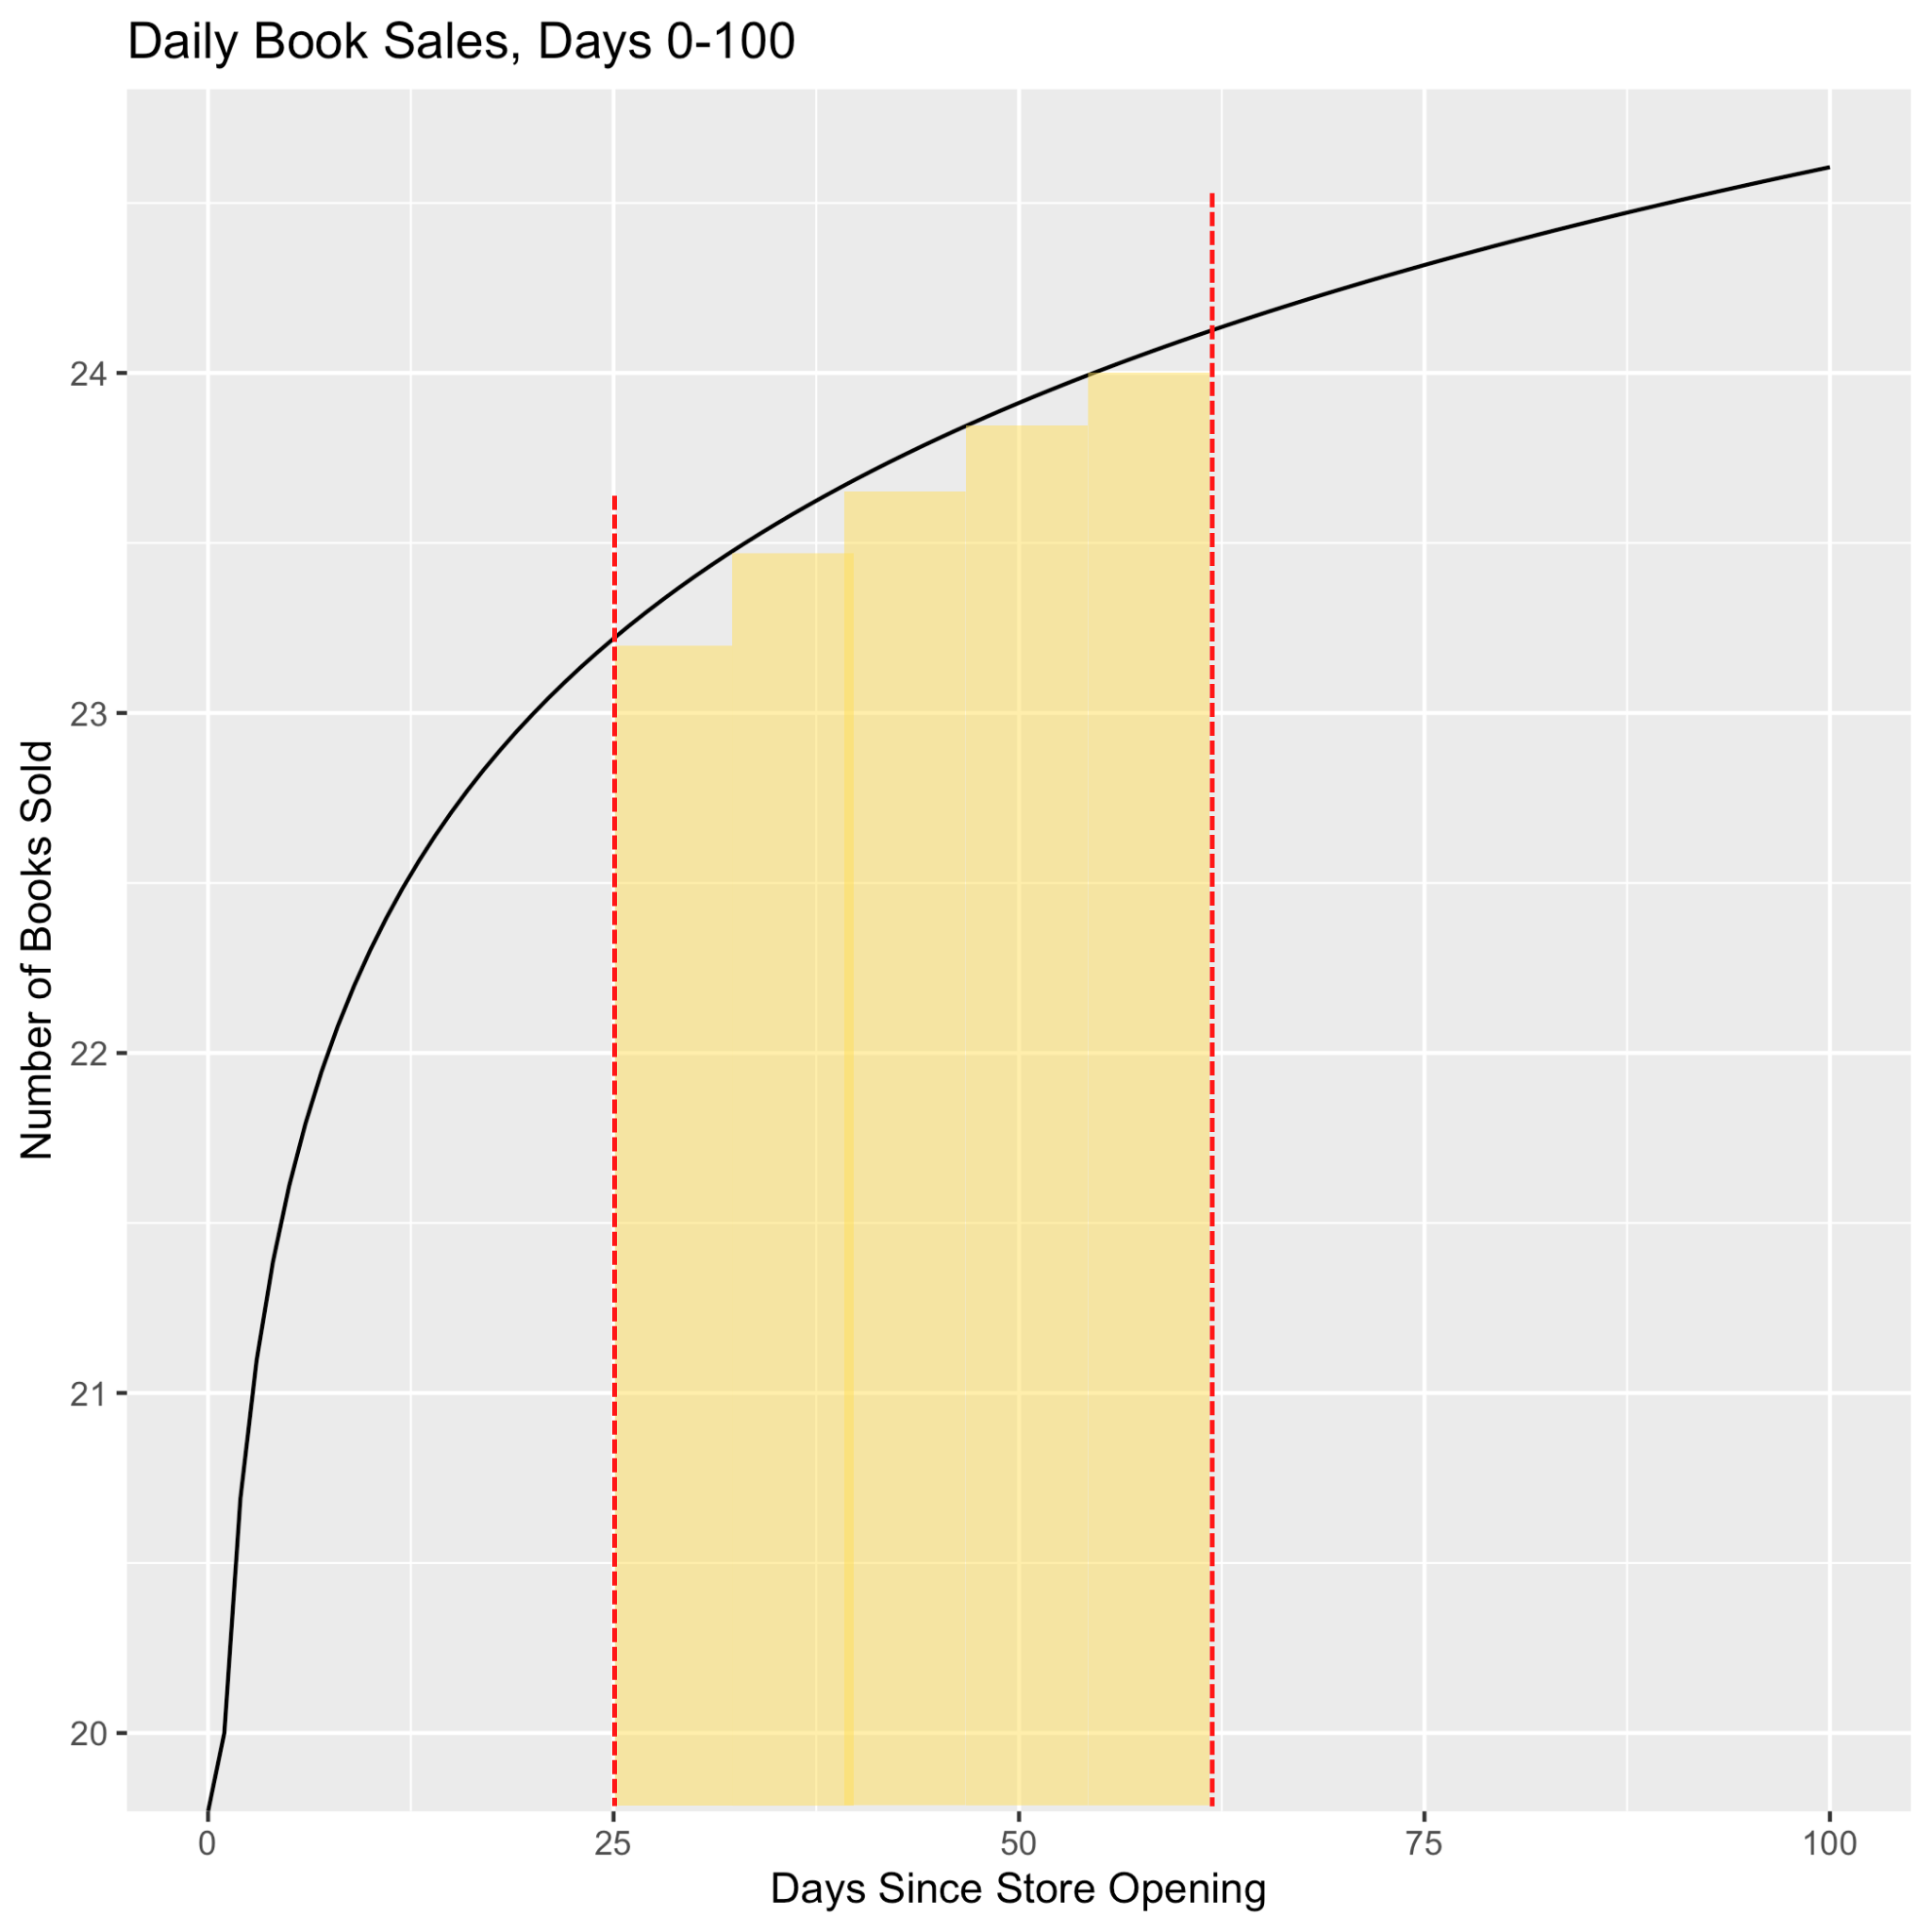
\includegraphics[width=0.5\textwidth,height=\textheight]{"~/OneDrive - Northwestern University/Teaching/2022_MathCamp/Proposed AM Slides/images/book_sales_interval.png"}
\end{frame}

\begin{frame}{Alternative?}
\protect\hypertarget{alternative}{}
\begin{itemize}
\item
  Instead, we can solve for the integral of this function to find the
  \emph{total or cumulative} area under the curve within some specified
  bounds.
\item
  This is much more precise and efficient.
\end{itemize}
\end{frame}

\begin{frame}{Integrals}
\protect\hypertarget{integrals}{}
\begin{itemize}[<+->]
\tightlist
\item
  Integrals are the inverse of derivatives. Where derivatives tell us
  about the marginal and instantaneous rate of change of a specific
  function, integrals are a
  \href{https://mathworld.wolfram.com/Integral.html}{generalization}.
  The generalization of the function means that we can learn about the
  area that the function encompasses.
\end{itemize}
\end{frame}

\begin{frame}{Indefinite Integrals and Anti-Derivatives}
\protect\hypertarget{indefinite-integrals-and-anti-derivatives}{}
\begin{itemize}[<+->]
\tightlist
\item
  \textbf{Indefinite Integrals} and \textbf{Anti-Derivatives} are terms
  that are essentially interchangeable.
\end{itemize}

\begin{itemize}[<+->]
\tightlist
\item
  Indefinite integrals assign an \textbf{integral} \(F(x)\) for the
  \textbf{integrand} \(f(x)\), wherein there are no limits on the
  integral. This means that we want to find the most general form of the
  integral.
\end{itemize}

\begin{itemize}[<+->]
\tightlist
\item
  The indefinite integral is given by \(\int f(x) dx = F(x) + c\),
  wherein \(\int\) is the integration operator, \(dx\) refers to the
  variable to be integrated (\(x\)), and \(c\) is a constant.
\end{itemize}

\begin{itemize}[<+->]
\tightlist
\item
  Indefinite integrals must always account for the constant \(c\).
  Remember the rules of differentiation regarding constants-- they go to
  0.
\end{itemize}
\end{frame}

\begin{frame}{Definite Integrals}
\protect\hypertarget{definite-integrals}{}
\begin{itemize}[<+->]
\tightlist
\item
  \textbf{Definite Integrals} are the same conceptually as indefinite
  integrals in that they give a function to be defined, however they
  place \emph{bounds} on the interval , \([a,b]\), of the integral.
\end{itemize}

\begin{itemize}[<+->]
\tightlist
\item
  \emph{How does this look in practice?} \pause An indefinite integral
  solves for an \emph{general equation} \(f(x)\), whereas a definite
  integral solves for a \emph{value}, or at least a function of
  difference between the upper and lower bounds.
\end{itemize}

\begin{itemize}[<+->]
\tightlist
\item
  In the case of a definite integral, we instead notate the integral as
  \(\int_a^b f(x)dx\). Notice that the bounds \(b\) and \(a\) notate the
  upper and lower bounds, respectively.
\end{itemize}
\end{frame}

\begin{frame}{The \emph{Anti}derivative}
\protect\hypertarget{the-antiderivative}{}
Ultimately the process of moving from derivatives to integrals should be
possible both forward and backward. This is to say, these processes are
inverse to each other and we \emph{should} be able to perform
differentation and anti-differentiation forward and backward.

This gives us the first fundamental theorem of calculus!!

\[ f'(x) \longleftrightarrow f(x) \longleftrightarrow F(x)\] Thus,
\(F'(x)= f(x)\)!
\end{frame}

\begin{frame}{Fundamental Theorem of Calculus}
\protect\hypertarget{fundamental-theorem-of-calculus}{}
\begin{itemize}[<+->]
\tightlist
\item
  We also want to use the definite integral to solve for the integral
  over a range of values, {[}a,b{]}. Mathematically this entails:
\end{itemize}

\[ \int_a^b f(x)dx = F(x) |^b_a = F(b)-F(a)\]

\begin{itemize}[<+->]
\tightlist
\item
  This is the more common recitation of the \textbf{fundamental theorem
  of calculus}. Without getting into too much math, this theorem states
  that with this information that we solve for the \emph{area under the
  functional curve over the stated interval}.
\end{itemize}

\begin{itemize}[<+->]
\tightlist
\item
  With a bounded integral, we can ditch the constant, \(c\), included in
  the indefinite integral because algebra will cancel it out.
\end{itemize}
\end{frame}

\begin{frame}{Why does it matter?}
\protect\hypertarget{why-does-it-matter}{}
As we will talk about more tomorrow, the ``area under the curve'' is
important for calculating probability.

Perhaps you all are familiar with the Bell Curve distribution, wherein
we can estimate the percentile of a given score based on its location on
within the curve.

This Bell Curve model is possible because of the information that
calculus reveals to us \emph{about} a probability distribution.
\end{frame}

\begin{frame}{OK\ldots{} so now how do I do it?}
\protect\hypertarget{ok-so-now-how-do-i-do-it}{}
\begin{itemize}[<+->]
\tightlist
\item
  Like derivatives, solving for integrals essentially comes down to a
  lot of rules. Solving for definite integrals also entails a bit of
  algebra.
\end{itemize}

\begin{itemize}[<+->]
\tightlist
\item
  Remember that the simple rule for calculating the derivative is
  \(\frac{dx^n}{dx} = nx^{n-1}\); furthermore, remember that we are
  trying to achieve the `original' function of f'(x) with the
  antiderivative.
\end{itemize}

\begin{itemize}[<+->]
\tightlist
\item
  Therefore, finding the integral requires that we obtain the inverse of
  the derivative. Finding the inverse implies that we will perform the
  opposite algebraic operation on the function. Furthermore, remember we
  must also account for a potential constant, \(c\).
\end{itemize}
\end{frame}

\begin{frame}{But really\ldots{} how do I do it?}
\protect\hypertarget{but-really-how-do-i-do-it}{}
\begin{itemize}[<+->]
\tightlist
\item
  When dealing with powers and basic integration:
\end{itemize}

\[ \frac{dx^n}{dx} = nx^{n-1} \rightarrow \int \frac{x^{n+1}}{n+1} + c\]

\begin{itemize}[<+->]
\tightlist
\item
  Note here that finding an integral in this form is not possible if
  \(n \neq -1\).
\end{itemize}
\end{frame}

\begin{frame}{Starting Out}
\protect\hypertarget{starting-out}{}
Given this simple rule, let's practice with a couple of functions.

Let's try to integrate the following:

\begin{itemize}
\tightlist
\item
  \(\int 3x + 3 dx\)
\end{itemize}

\uncover<2->{\color{blue}\hspace{2cm} $F(x) = \frac{3}{2}x^2 + 3x +c$}

\begin{itemize}
\tightlist
\item
  \(\int 16x^2 + 2x + 7 dx\)
\end{itemize}

\uncover<3->{\color{blue}\hspace{2cm}$F(x)= \frac{16}{3}x^3 + x^2 + 7x + c$}

\begin{itemize}
\tightlist
\item
  \(\int \sqrt{x} + 13 dx\)
\end{itemize}

\uncover<4->{\color{blue}\hspace{2cm} $F(x)= \frac{2}{3}x^{\frac{3}{2}} + 13x + c$}
\end{frame}

\begin{frame}{Integration as a Linear Operator}
\protect\hypertarget{integration-as-a-linear-operator}{}
This has a few
\href{https://math.mit.edu/~jorloff/suppnotes/suppnotes01-01a/01pi.pdf}{implications:}

\begin{enumerate}
\tightlist
\item
  \(\int^b_a (f(x)\pm g(x))dx = \int^b_a f(x)dx \pm \int^b_a g(x)dx\)
\end{enumerate}

\begin{itemize}[<+->]
\tightlist
\item
  This means that the sum/difference of two functions \(f\) and \(g\)
  integrated is equal to the sum/difference of their individual
  integration.
\end{itemize}

\begin{enumerate}
\setcounter{enumi}{1}
\tightlist
\item
  \(\int^b_a Cf(x)dx = C\int^b_a f(x)dx\)
\end{enumerate}

\begin{itemize}[<+->]
\tightlist
\item
  The integral of a function scaled by a constant is equal to the
  constant times the integral.
\end{itemize}
\end{frame}

\begin{frame}{Practice}
\protect\hypertarget{practice}{}
Let's see how those two properties play out:

\begin{itemize}[<+->]
\tightlist
\item
  \(\int^2_0 (x+2) + (2x-7) dx\)
\end{itemize}

\uncover<2->{$\int^2_0 (x+2) dx + \int^2_0 (2x-7)dx$}

\uncover<3->{$ \frac{1}{2}x^2 + 2x |^2_0 + x^2 -7 |^2_0 $}

\uncover<4->{$[(\frac{1}{2}(2)^2 + 2(2)) - 0] - [((2)^2-7(2))-0]$ }

\uncover<5->{$= -4$}
\end{frame}

\begin{frame}{Practice}
\protect\hypertarget{practice-1}{}
\begin{itemize}[<+->]
\tightlist
\item
  \(\int^2_0 4(x+2) dx\)
\end{itemize}

\uncover<2->{$4 \int^2_0 (x+2) dx$}

\uncover<3->{$4 [\frac{1}{2}x^2 +2x |^2_0]$}

\uncover<4->{$4 [6-0] = 24$}
\end{frame}

\begin{frame}{More on Integrals}
\protect\hypertarget{more-on-integrals}{}
There are more properties that will become somewhat self evident as long
as you have more practice with them.

Beyond this though is continuing to address how to solve them. There are
two ways of handling integrals, which are ultimately a bit more hard to
deal with than derivatives.

\begin{itemize}
\item
  Integration by Substitution:
\item
  Integration by Parts
\item
  Integration given Trigonometric Identities
\end{itemize}

We can also have multiple integrals with multiple variables.

\[ \int_c^d \int_a^b f(x,y) dxdy\]
\end{frame}

\begin{frame}{The Fun Part Is\ldots.}
\protect\hypertarget{the-fun-part-is.}{}
\begin{itemize}
\item
  You probably won't have to do any of these calculations. Unless you go
  onto more advanced stats classes.
\item
  So we won't cover solving for them extensively here.
\end{itemize}
\end{frame}

\begin{frame}{Here's some more practice based on what we have learned so
far}
\protect\hypertarget{heres-some-more-practice-based-on-what-we-have-learned-so-far}{}
Solve for the following, be sure to pay attention whether the integral
is definite or indefinite: \small 

\begin{enumerate}
\tightlist
\item
  \(\int(x^3-x^2+2x)dx\)
\end{enumerate}

\uncover<2->{\color{blue} \hspace{2cm}$F(x)= \frac{x^4}{4}-\frac{x^3}{3}+x^2+c$}

\begin{enumerate}
\setcounter{enumi}{1}
\tightlist
\item
  \(\int^5_1 \frac{1}{x^3}dx\)
\end{enumerate}

\uncover<3->{\color{blue} \hspace{2cm}$-\frac{1}{2x^2}|^5_1=0.48$}

\begin{enumerate}
\setcounter{enumi}{2}
\tightlist
\item
  \(\int^5_1 x^3+ \frac{1}{x^3}dx\)
\end{enumerate}

\uncover<4->{\color{blue} \hspace{2cm}$\frac{1}{4}x^4|^5_1 + (-\frac{1}{2x^2}|^5_1)= 156.48 \hspace{0.5cm} \text{or} \hspace{0.5cm} \frac{3912}{25}$}

\begin{enumerate}
\setcounter{enumi}{3}
\tightlist
\item
  \(\int^{1}_0 e^x dx\) \textbf{hint: the integral of \(e^x\) is the
  same as its derivative.}
\end{enumerate}

\uncover<5->{\color{blue} \hspace{2cm}$e^x|^1_0 = (e-1) \hspace{0.5cm} \text{or} \hspace{0.5cm} 1.7183$}
\end{frame}

\end{document}
